\textbf{\underline{OZ 2 - Magnetische velden - Oefening 4:}}
\vspace{0.5cm}

Een draad van 4,00 m met massa 0,100 kg wordt gebruikt om een vierkante spoel met zijde 0,100 m te maken. De spoel wordt opgehangen aan ëën van zijn horizontale zijden in een verticaal magnetisch veld van 0,0100 T. Vervolgens stuurt men een stroom van 3,40 A door de spoel. Bepaal de hoek die de spoel maakt met de verticale wanneer de spoel zijn evenwichtspositie heeft bereikt. Wat is het krachtmoment (torsie) die het magnetisch veld op de spoel uitoefent in deze situatie?

\begin{description}[labelwidth=1.5cm, leftmargin=!]
    \item[Geg. :]   $ l = 4,00 $ m; $ m = 0,100 $ kg; $ z = 0,100 $ m; $ B = 0,0100 $ T; $ I = 3,40 $ A;
        % \begin{figure}[H]
        %     \centering
        %     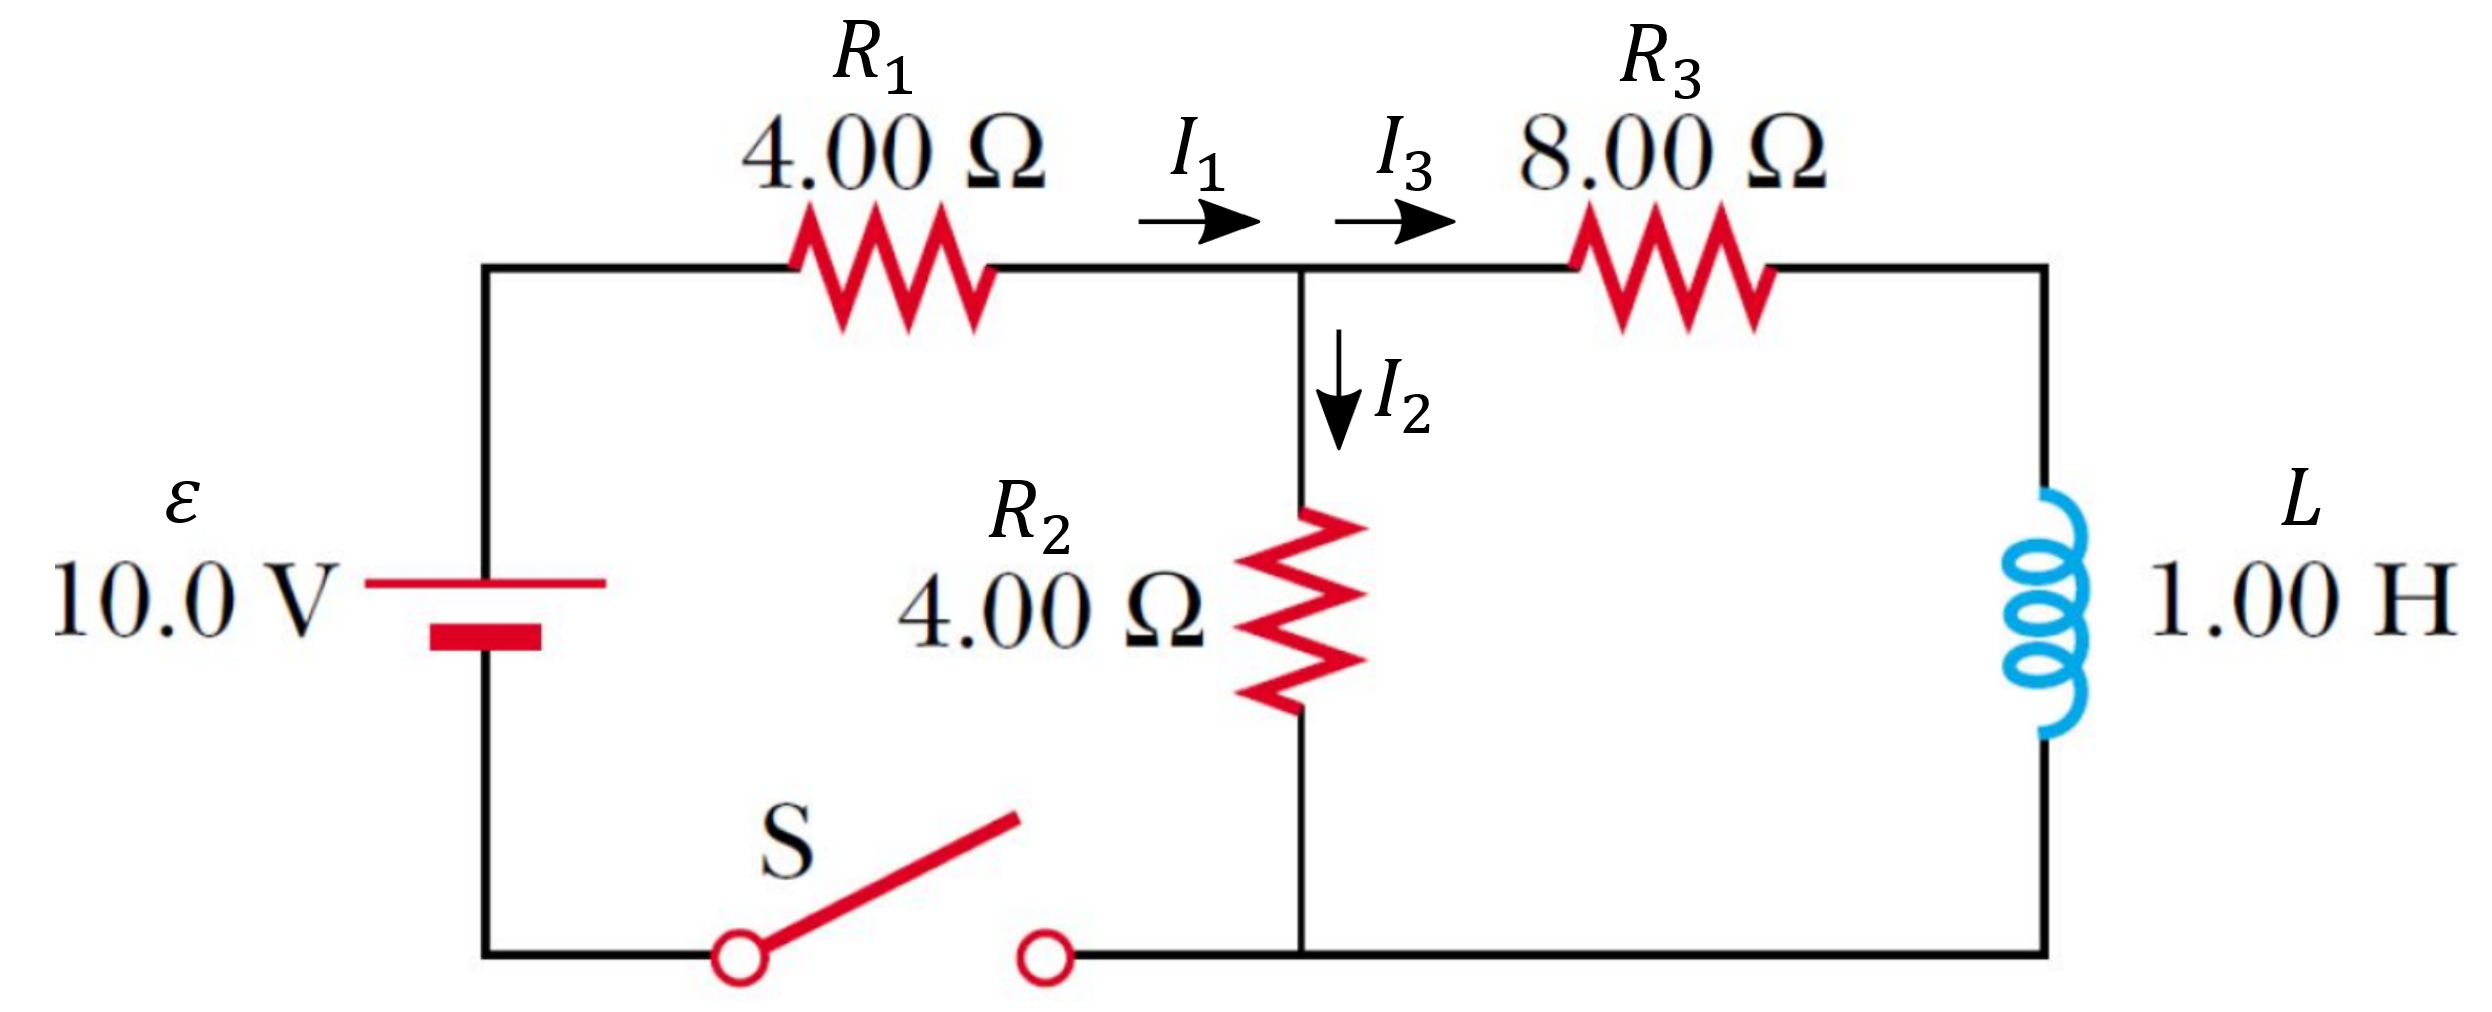
\includegraphics[width=8cm]{oz02/resources/oef-4-schets.png}
        % \end{figure}
    \item[Gevr. :]  $ \theta_e $; $ M_e $;
    \item[Opl. :] 
    (Oplossing van Serway 6E Chapter 29 Problem 22)

(a) Let $\theta$ represent the unknown angle; $L$, the total length of the wire; and $d$, the length of one side of the square coil. Then, using the definition of magnetic moment and the right-hand rule in Figure 29.15, we find
\\\\
$\mu=N A I$ :
$\boldsymbol{\mu}=\left(\frac{L}{4 d}\right) d^2 I$ at angle $\theta$ with the horizontal.
\\\\
At equilibrium,
$\sum \boldsymbol{\tau}=(\boldsymbol{\mu} \times \mathbf{B})-(\mathbf{r} \times m \mathbf{g})=0$
\\
$\left(\frac{I L B d}{4}\right) \sin \left(90.0^{\circ}-\theta\right)-\left(\frac{m g d}{2}\right) \sin \theta=0$
\\\\
and
$$
\begin{aligned}
& \left(\frac{m g d}{2}\right) \sin \theta=\left(\frac{I L B d}{4}\right) \cos \theta \\
& \theta=\tan ^{-1}\left(\frac{I L B}{2 m g}\right)=\tan ^{-1}\left(\frac{(3.40 \mathrm{~A})(4.00 \mathrm{~m})(0.0100 \mathrm{~T})}{2(0.100 \mathrm{~kg})\left(9.80 \mathrm{~m} / \mathrm{s}^2\right)}\right)=3.97^{\circ} .
\end{aligned}
$$
(b) $\quad \tau_m=\left(\frac{I L B d}{4}\right) \cos \theta=\frac{1}{4}(3.40 \mathrm{~A})(4.00 \mathrm{~m})(0.0100 \mathrm{~T})(0.100 \mathrm{~m}) \cos 3.97^{\circ}=3.39 \mathrm{mN} \cdot \mathrm{m}$
\end{description}

\vspace{1cm}